\section{Applications and Setups}
We apply \cws and \fwl, two approaches introduced in this chapter for learning from vast amount of weakly annotated data, while a small set of labeled data exist, to two different tasks: \emph{document ranking} and \emph{sentiment classification}. 
Whilst these two applications differ considerably, as do the exact operationalization of the propose models to these cases, in both cases the human gold standard data is based on a cognitively complex, or subjective, judgments causing high interrater variation, increasing both the cost of obtaining labels as the need for larger sets of labels.

\begin{table}[tbp]
\caption{\label{tbl_baselines} Descriptions of baseline models.
}
\centering
\fontsize{10}{12}\selectfont{
% \begin{adjustbox}
{\renewcommand{\arraystretch}{1.4}
\begin{tabular}{@{}l@{~~}p{0.18\textwidth}@{~~~~}p{0.9\textwidth}@{}}
\toprule
\multicolumn{3}{c}{\textbf{Basic Baselines}}
\\\midrule
1 & \textbf{WA} & The \wa, i.e. the unsupervised method used for annotating the unlabeled data.
\\
2 & \textbf{$\text{NN}_{\text{S}}$} & Full Supervision Only, i.e. the \tnet (or the \std) trained only on strong labeled data ($\mathcal{D}_s$).
\\
3 & \textbf{$\text{NN}_{\text{W}}$} &  Weak Supervision Only, i.e. the \tnet (or the \std)  trained only on weakly labeled data ($\mathcal{D}_w$).
\\ \midrule
4 & \textbf{$\text{NN}_{\text{W}\text{/S}^+}$}  & Weak Supervision + Oversampled Strong Supervision, i.e. the \tnet (or the \std) trained on samples that are alternately drawn from $\mathcal{D}_w$ without replacement, and $\mathcal{D}_s$ with replacement. Since $|\mathcal{D}_s| \ll |\mathcal{D}_w|$, it oversamples the strong data.
\\
5 & \textbf{$\text{NN}_{\text{W}} \to \text{NN}_{\text{S}}$}  & Weak Supervision + Fine Tuning, i.e. the \tnet (or the \std) trained on weak dataset $\mathcal{D}_w$ and fine-tuned on strong dataset $\mathcal{D}_s$.
\\
6 & \textbf{$\text{NN}_{\text{W}} \to \text{NN}^{\text{Sup}}_{\text{S}}$} & Weak Supervision + Supervision Layer Fine-Tuning, i.e. the \tnet (or the \std) trained only on on weak dataset $\mathcal{D}_w$ and the supervision layer is fine-tuned on strong dataset $\mathcal{D}_s$, while the representation learning layer is kept fixed.
\\
7 & \textbf{$\text{NN}_{\text{W}} \to \text{NN}^{\text{Rep}}_{\text{S}}$} & Weak Supervision + Representation Learning Layer Fine Tuning, i.e. the \tnet (or the \std) trained only on on weak dataset $\mathcal{D}_w$ and the representation layer is fine-tuned on strong dataset $\mathcal{D}_s$, while the representation learning layer is kept fixed.
\\\midrule
\multicolumn{3}{c}{\textbf{Controlled Weak Supervision baselines}}
\\\midrule
8 & \textbf{\cws} & Learning from Controlled Weak Supervision that is explained in Section~\ref{sec:meta_learning}.
\\
9 & \textbf{\cws$_\text{JT+}$} & Controlled Weak Supervision with Joint Training is the same as \cws (explained in Section~\ref{sec:modeltraining}), except that parameters of the supervision layer in \tnet are also updated using batches from $V$, with regards to the strong labels.
\\
10 & \textbf{\cws$_\text{ST}$} & Separate Training, i.e. we consider the \cnet as a separate network, without sharing the representation learning layer, and train it on set $V$. We then train the \tnet on the controlled weak supervision signals.
\\
11 & \textbf{\cws$_\text{CT}$} & Circular Training, i.e. we train the \tnet on set $U$. Then the \cnet is trained on data with strong labels, and the \tnet is trained again but on controlled weak supervision signals.
\\
12 & \textbf{\cws$_\text{PT}$} & Progressive Training is the mixture of the two previous baselines. Inspired by \cite{Rusu:2016}, we transfer the learned information from the converged \tnet to the \cnet using progressive training. We then train the \tnet again on the controlled weak supervision signals.
\\\midrule
\multicolumn{3}{c}{\textbf{Fidelity Weighted Learning baselines}}
\\\midrule
13 & \textbf{\fwl} & Fidelity Weighted Learning that is explained in Section~\ref{sec:fidelity_weighted_learning}.
\\
14 & \textbf{$\text{NN}_{\text{W}^\omega \to \text{NN}_\text{S}}$} & The \std trained on the weak data, but the step-size of each weak sample is weighted by a fixed value $0 \leq \omega \leq 1$, and fine-tuned on strong data. As an approximation for the optimal value for $\omega$, we have used the mean of $\eta_2$ of our model (below).
\\
15 & \textbf{\fwl$_{unsuprep}$} & The representation in the first step is trained in an unsupervised way\footnote{In the document ranking task, as the representation of documents and queries, we use weighted averaging over pretrained embeddings of their words based on their inverse document frequency~\citep{Dehghani:2017:SIGIR}. In the sentiment analysis task, we use skip-thoughts vectors\citep{kiros2015skip}} and the student is trained on examples labeled by the \tch using the confidence scores.
\\
16 & \textbf{\fwl$\backslash\Sigma$} & The \std trained on the weakly labeled data and fine-tuned on examples labeled by the \tch without taking the confidence into account. This baseline is similar to \citep{Veit:2017}.
\\\bottomrule
\end{tabular}
}
}
%\end{adjustbox}
\end{table}


For both tasks, we evaluate the performance of \cws as well as \fwl compared to some baselines that are described in Table~\ref{tbl_baselines}. 
%We also conducted a series of ablation studies.

\subsection{Document Ranking}
This task is the core information retrieval problem and is challenging as the ranking model needs to learn a representation for long documents and capture the notion of relevance between queries and documents. Furthermore, as it was discussed in Chapter~\ref{chap:4}, the size of publicly available datasets with query-document relevance judgments is unfortunately quite small ($\sim 250$ queries).
%
In our experiments, ranking is cast as a regression task. Given each training sample $x$ as a triple of query $q$, and two documents $d^+$ and $d^-$, the goal is to learn a function $\mathcal{F} : \{<q, d^+, d^->\} \rightarrow \mathbb{R}$, which maps each data sample $x$ to a scalar output value $y$ indicating the probability of $d^+$ being ranked higher than $d^-$ with respect to $q$. 

\begin{figure}{t}
    \centering
            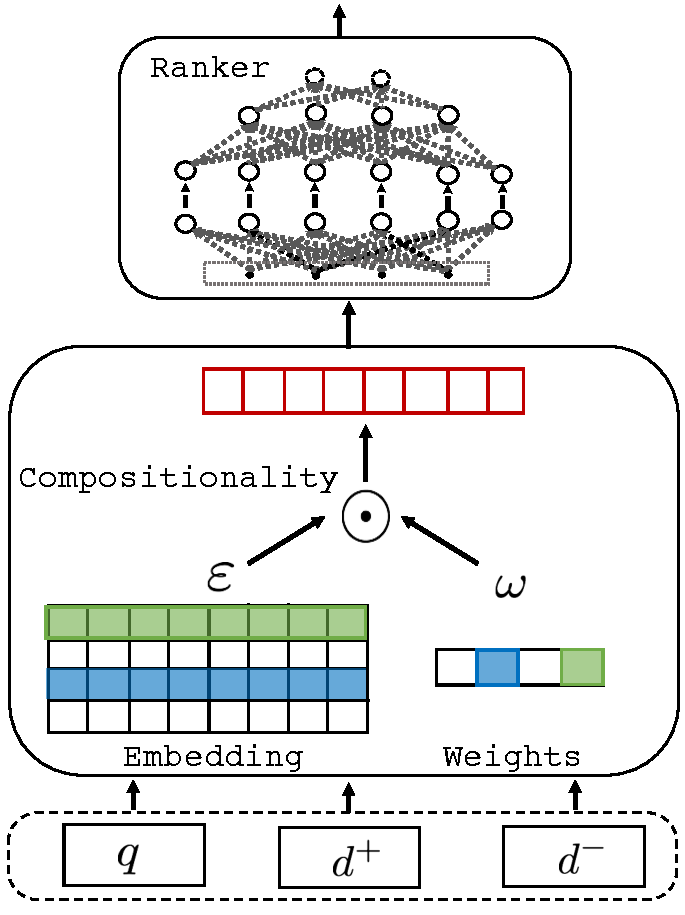
\includegraphics[width=0.35\textwidth]{03-part-02/chapter-05/figs_and_tables/fig_ranker.pdf}
    \caption{The document ranker used as \tch in \cws and \std in \fwl.}
    \label{fig:ranker}
\end{figure}


\subsubsection{The \tnet in \cws and the \std in \fwl}
We employ the pairwise neural ranker architecture explained in Section~\ref{sec:modeltwo} as the \tnet in \cws and \std in \fwl. 

Each training instance $x$ consists of a query $q$, and two documents $d^+$ and $d^-$. The labels, $\tilde{y}$ and $y$, are scalar values indicating the probability of $d^+$ being ranked higher than $d^-$ with respect to $q$.

\mypar{The Representation Learning Layer.}
This layer learns a function $\varepsilon: \mathcal{V} \rightarrow \mathbb{R}^{m}$  (where $\mathcal{V}$ denotes the vocabulary set, and $m$ is the number of embedding dimensions) that maps each word to its embedding which is downstream of the ranking task as well as a weighting function $\omega: \mathcal{V} \rightarrow \mathbb{R}$ which learns the global importance of each word. Then, the learned weights are used to compose word embeddings to generate query/document embeddings. The output of this layer is the concatenation of vectors representing query and two documents.
%
In our experiments, we initialize the embedding function $\varepsilon$ with word2vec embeddings~\cite{Mikolov:2013} pre-trained on Google News and the weighting function $\omega$ with IDF.

\mypar{The Supervision Layer.} 
This layer receives the vector representation of the inputs processed by the representation learning layer and outputs a prediction $\hat{y}_i$.
We opt for a simple fully connected feed-forward network with $l$ hidden layers followed by a sigmoid. We employ the weighted cross entropy loss:
\begin{equation}
% \nonumber
\small
\mathcal{L}_t = \sum_{i\in B_U} \tilde{c}_i [- \tilde{y}_i \log (\hat{y}_i) - (1-\tilde{y}_i) \log(1-\hat{y}_i)],
\end{equation}
where $B_U$ is a batch of instances from $U$, and $\tilde{c}_i$ is the confidence score of the weakly annotated instance $i$, estimated by the \cnet.

The general schema of the \tnet (or \std) is illustrated in Figure~\ref{fig:ranker}. More details are provided in Section~\ref{sec:modeltwo}.

\subsubsection{The \wa}
The \wa in the document ranking task is BM25~\citep{Robertson:2009}, a well-known unsupervised retrieval method. This method heuristically scores a given pair of query-document based on the statistics of their matched terms. In the pairwise document ranking setup, $\tilde{y}_i$ for a given sample $x_j = (q,d^+,d^-)$ is the probability of document $d^+$ being ranked higher than $d^-$: 
$\tilde{y}_i = P_{q,d^+,d^-} = \nicefrac{s_{q,d^+}}{s_{q,d^+} + s_{q,d^-}}$,  where $s_{q,d}$ is the score obtained from the \wa.


\subsubsection{The \cnet in \cws}
The \cnet is a regresses and we use a simple fully connected feed-forward network. To train the \cnet, the target label $c_j$ is calculated using the absolute difference of the strong label and the weak label: $c_j= 1-|y_j - \tilde{y}_j|$, where $y_j$ is calculated similar to $\tilde{y}_i$, but $s_{q,d}$ comes from strong labels provided by humans.


\subsubsection{The \tch in \fwl}
We use Gaussian Process as the \tch in order to generate soft labels. We pass the mean of $\mathcal{GP}$ through the same function $g(.)$ that is applied on the output of the \std network, where the $g(.)$ is sigmoid for the document ranking task.
Since we have one dimensional regression here, $\Sigma(x_t)$ is scalar and $h(.)$ is identity.
In the \tch, linear combinations of different kernels are used. For the document ranking task, we use sparse variational GP regression\footnote{\url{http://gpflow.readthedocs.io/en/latest/notebooks/SGPR_notes.html}}~\citep{Titsias2009variational} with this kernel:
\begin{equation}
k(x_i,x_j)=k_{\rm Matern3/2}(x_i,x_j)+{k_{\rm Linear}}(x_i,x_j)+k_{\rm White}(x_i,x_j)
\end{equation}

where,
\begin{flalign*}
    \hspace{6em}
    &&k_{\rm Matern3/2}(x_i,x_j) &= \left(1+\frac{\sqrt{3}\Vert x_i-x_j\Vert}{l}\right)\exp{\left(-\frac{\sqrt{3}\Vert x_i-x_j\Vert}{l}\right)} & \\
    &&k_{\rm Linear}(x_i,x_j) &= \sigma_0^2+x_i.x_j & \\
    &&k_{\rm White}(x_i,x_j) &= constant\_value, \quad \forall x_1=x_2 \text{ and } 0 \text{ otherwise} & 
\end{flalign*}

We empirically found $l=1$ satisfying value for the length scale of Matern3/2 kernel.
We also set $\sigma_0 = 0$ to obtain a homogeneous linear kernel. 
The constant value of $K_{White}(.,.)$ determines the level of noise in the labels. This is different from the noise in weak labels. This term explains the fact that even in strong labels there might be a trace of noise due to the inaccuracy of human labelers. 

It's noteworthy that we used clustered $\mathcal{GP}$ algorithm, explained in Section~\ref{sec:CGP}, and set the number of clusters to $50$ for this task..  


\subsubsection{Collections}
We use two standard TREC collections for the task of ad-hoc retrieval: The first collection (\emph{Robust04}) consists of 500k news articles from different news agencies as a homogeneous collection. The second collection (\emph{ClueWeb}) is ClueWeb09 Category B, a large-scale web collection with over 50 million English documents, which is considered as a heterogeneous collection. Spam documents were filtered out using the Waterloo spam scorer~\footnote{\url{http://plg.uwaterloo.ca/~gvcormac/clueweb09spam/}}~\citep{Cormack:2011} with the default threshold $70\%$. 

\mypar{Data with strong labels.} 
We take query sets that contain human-labeled judgments: a set of 250 queries (TREC topics 301--450 and 601--700) for the Robust04 collection and a set of 200 queries (topics 1-200) for the experiments on the ClueWeb collection.
For each query, we take all documents judged as relevant plus the same number of documents judged as non-relevant and form pairwise combinations among them.

\mypar{Data with weak labels.}
We create a query set $Q$ using the unique queries appearing in the AOL query logs~\citep{Pass:2006}. 
This query set contains web queries initiated by real users in the AOL search engine that were sampled from a three-month period from March 2006 to May 2006. 
We applied standard pre-processing~\cite{Dehghani:2017:SIGIR,Dehghani2017:CIKM} on the queries: We filtered out a large volume of navigational queries containing URL substrings (``http'', ``www.'', ``.com'', ``.net'', ``.org'', ``.edu''). We also removed all non-alphanumeric characters from the queries. For each dataset, we took queries that have at least ten hits in the target corpus using our \wa method. Applying all these steps, 
We collect 6.15 million queries to train on in Robust04 and 6.87 million queries for ClueWeb.
To prepare the weakly labeled training set $\mathcal{D}_w$, we take the top $1,000$ retrieved documents using BM25 for each query from training query set $Q$, which in total leads to $\sim|Q|\times 10^6$ training samples. 

\subsubsection{Experimental Setup.}
For the evaluation of the whole model, we conducted a 3-fold cross-validation. However, for each dataset, we first tuned all the hyper-parameters of the \tnet in \cws (and \std in the first step of \fwl) in the first step on the set with strong labels using batched GP bandits with an expected improvement acquisition function~\citep{Desautels:2014} and kept the optimal parameters of the \tnet (and \std) fixed for all the other experiments.
The size and number of hidden layers for the \tnet (and \std) is selected from $\{64, 128, 256, 512\}$. The initial learning rate and the dropout parameter were selected from $\{10^{-3}, 10^{-5}\}$ and $\{0.0, 0.2, 0.5\}$, respectively. We considered embedding sizes of $\{300, 500\}$. The batch size in our experiments was set to $128$.  We use ReLU~\citep{Nair:2010} as a non-linear activation function $\alpha$ in \tnet (and \std).  We use the Adam optimizer~\citep{Kingma:2014} for training, and \emph{dropout}~\citep{Srivastava:2014} as a regularization technique.

%
At inference time, for each query, we take the top $2,000$ retrieved documents using BM25 as candidate documents and re-rank them using the trained models. We use the Indri\footnote{\url{https://www.lemurproject.org/indri.php}} implementation of BM25 with default parameters (i.e., $k_1 = 1.2$, $b = 0.75$, and $k_3 = 1,000$).

\subsubsection{Results and Discussions} 
\label{sec:res_and_disc_ranking}
We conducted k-fold cross validation on $\mathcal{D}_s$ (the strong data) and report two standard evaluation metrics for ranking: mean average precision (MAP) of the top-ranked $1,000$
documents and normalized discounted cumulative gain calculated for the top $20$ retrieved documents (nDCG@20). 
Table~\ref{tbl_main} shows the performance on both datasets. As can be seen, \fwl and \cws both provide significant boost on the performance on top of the baseline methods over both datasets.


\begin{table}[tbp]
\renewcommand{\arraystretch}{1.1}
\caption{\label{tbl_main}Performance of \cws and \fwl as well as the main baseline methods, described in Table~\ref{tbl_baselines}, for the document ranking task. \pssmall{i} indicates that the improvements with respect to the baseline $i$ are statistically significant at the 0.05 level using the paired two-tailed t-test with Bonferroni correction.}
\centering
\begin{adjustbox}{max width=\textwidth}
\begin{tabular}{r l l l l l}
\toprule
& \multirow{2}{*}{Method} &
\multicolumn{2}{c}{Robust04} & \multicolumn{2}{c}{ClueWeb}
\\ 
\cmidrule(lr){3-4} \cmidrule(lr){5-6}
& & \small{MAP} & \small{nDCG@20}
& \small{MAP} & \small{nDCG@20}
\\ \midrule
1 & \small{WA$_\text{BM25}$} 
& 0.2503\pssmall{2} & 0.4102\pssmall{2}  
& 0.1021\pssmall{2} & 0.2070\pssmall{2}
\\ \midrule
2 & \small{$\text{NN}_{\text{S}}$} 
& 0.1790 & 0.3519  
& 0.0782 & 0.1730
\\
3 & \small{$\text{NN}_{\text{W}}$} 
& 0.2702\pssmall{12} & 0.4290\pssmall{12}  
& 0.1297\pssmall{12} & 0.2201\pssmall{12}
\\ \midrule
4 & \small{$\text{NN}_{\text{W}\text{/S}^+}$} 
&  0.2763\pssmall{123} & 0.4330\pssmall{123} 
&  0.1354\pssmall{123} & 0.2319\pssmall{123}
\\
5 & \small{$\text{NN}_{\text{W}} \to \text{NN}_{\text{S}}$} 
&  0.2810\pssmall{12346} & 0.4372\pssmall{12346} 
&  0.1346\pssmall{12346} & 0.2317\pssmall{12346}
\\
6 & \small{$\text{NN}_{\text{W}} \to \text{NN}^{\text{Sup}}_{\text{S}}$}
&  0.2711\pssmall{123} & 0.4203\pssmall{123} 
&  0.1002\pssmall{123} & 0.1940\pssmall{123}
\\
7 & \small{$\text{NN}_{\text{W}} \to \text{NN}^{\text{Rep}}_{\text{S}}$}
&  0.2810\pssmall{1234} & 0.4316\pssmall{1234} 
&  0.1286\pssmall{1234} & 0.2240\pssmall{1234}
\\
8 & \small{\cws}
&  0.3017\pssmall{1234567} & 0.4511\pssmall{1234567} 
&  0.1363\pssmall{1234567} & 0.2444\pssmall{1234567}
\\
13 & \small{\fwl}
& \textbf{0.3124}\pssmall{1234567}  & \textbf{0.460}\pssmall{1234567} & \textbf{0.1472}\pssmall{1234567}  & \textbf{0.2453}\pssmall{1234567}
\\\bottomrule
\end{tabular}
\end{adjustbox}
\end{table}



In the ranking task, the \std is designed in particular to be trained on weak annotations~\citep{Dehghani:2017:SIGIR}, hence training the network only on weak supervision, i.e. $\text{NN}_{\text{W}}$ performs better than $\text{NN}_{\text{S}}$. This can be due to the fact that ranking is a complex task requiring many training samples to learn representations that can be used to assess the relevance, while relatively few data with strong labels are available.

Alternating between strong and weak data during training, i.e. $\text{NN}_{\text{W}\text{/S}^+}$ seems to bring little (but statistically significant) improvement. However, we can gain better results by the typical fine-tuning strategies.  Among the fine-tuning experiments, updating all the parameters of the \tnet (or \std), i.e. $\text{NN}_{\text{W}} \to \text{NN}_{\text{S}}$, is the best fine-tuning strategy. Updating only the parameters of the representation layer based on the strong labels, i.e. $\text{NN}_{\text{W}} \to \text{NN}^{\text{Rep}}_{\text{S}}$, works better than updating only parameters of the supervision layer, i.e. $\text{NN}_{\text{W}} \to \text{NN}^{\text{Sup}}_{\text{S}}$. This supports our designed choice of a shared embedding layer in \cws which gets updated on set $V$.

\fwl is the best performing baselines, and \cws achieves 97\% of the performance of \fwl. The main advantage of \cws over \fwl is that it is trained in a single stage process and needs to meet the examples in $\mathcal{D}_w$ (which is a reasonably large set) only one time, while \fwl has three sequential stages during training and it needs to iterate two times over all the examples in $\mathcal{D}_w$. Also employing a Gaussian Process as part of the model in \fwl limits its scalability, while the components of \cws are all neural networks, and this eases the increase in the capacity of the model. 
% With all that, we find \cws a much more efficient model in terms of training cost, with losing little to no performance.


\begin{table}[tbp]
% \renewcommand{\arraystretch}{1.1}
\caption{\label{tbl_variants_rank_cws}Performance of the variants of the \cws on different datasets for document ranking task. Baselines are described in Table~\ref{tbl_baselines}.}
\centering
\begin{adjustbox}{max width=\textwidth}
\begin{tabular}{r l c c c c}
\toprule
& \multirow{2}{*}{\textbf{Method}} &
\multicolumn{2}{c}{\textbf{Robust04}} & \multicolumn{2}{c}{\textbf{ClueWeb}}
\\ 
\cmidrule(lr){3-4} \cmidrule(lr){5-6}
& & \small{\textit{MAP}} & \small{\textit{nDCG@20}}
& \small{\textit{MAP}} & \small{\textit{nDCG@20}}
\\ \midrule
\bf 8 & \bf \small{\cws}
&  \textbf{0.3017} & \textbf{0.4511}
&  0.1363 & \textbf{0.2444}
\\
\bf 9 & \bf \small{CWS$_\text{JT}^+$} 
& 0.2786  & 0.4367  
& 0.1310  & 0.2244 
\\ 
\bf 10 & \bf \small{CWS$_\text{ST}$} 
&  0.2716  & 0.4237 
&  0.1320  & 0.2213
\\
\bf 11 & \bf \small{\cws$_\text{CT}$} 
&  0.2961 & 0.4440 
&  \textbf{0.1378}  & 0.2431 
\\ 
\bf 12 & \bf \small{\cws$_\text{PT}$} 
& 0.2784  & 0.4292  
& 0.1314  & 0.2207
\\\bottomrule
\end{tabular}
\end{adjustbox}
\end{table}


As an ablation study on \cws, we tried different training strategies and report the results in Table~\ref{tbl_variants_rank_cws}. As shown, \cws and CWS$_\text{CT}$ perform better than other strategies.
%
\cws$_\text{CT}$ is to let the \cnet to be trained separately, while still being able to enjoy shared learned information from the \tnet. Compared to \cws, \cws$_\text{CT}$ is less efficient as we need two rounds of training on weakly labeled data. 

While it seems reasonable to make use of strong labels for updating \emph{all} parameters of the \tnet, CWS$_\text{JT}^+$ achieves no better results than \cws. We speculate that during training, the direction of the parameter optimization is profoundly affected by the type of supervision signal and while we control the magnitude of the gradients, we do not change their directions. Hence alternating between two sets with different label qualities (different supervision signal types, i.e. weak and strong) confuses the supervision layer of the \tnet. 

In \cws$_\text{ST}$,  the strong dataset, $\mathcal{D}_s$, is too small to train a high-quality \cnet without taking advantage of the vast amount of weakly annotated data in $\mathcal{D}_w$ to learn better representations, so CWS$_\text{ST}$ is not able to improve the performance over $\text{NN}_W$ significantly and also we noticed that this strategy leads to a slow convergence compared to the $\text{NN}_W$. 
Also transferring learned information from \tnet to \cnet via progressive training, i.e., CWS$_\text{PT}$, performs no better than full sharing of the representation learning layer.



\begin{table}[tbp]
% \renewcommand{\arraystretch}{1.1}
\caption{\label{tbl_variants_rank_fwl}Performance of \fwl against some of the baselines on different datasets for document ranking task. Baselines are described in Table~\ref{tbl_baselines}.}
\centering
\begin{adjustbox}{max width=\textwidth}
\begin{tabular}{r l c c c c}
\toprule
& \multirow{2}{*}{\textbf{Method}} &
\multicolumn{2}{c}{\textbf{Robust04}} & \multicolumn{2}{c}{\textbf{ClueWeb}}
\\ 
\cmidrule(lr){3-4} \cmidrule(lr){5-6}
& & \small{\textit{MAP}} & \bf \small{\textit{nDCG@20}}
&  \small{\textit{MAP}} & \bf \small{\textit{nDCG@20}}
\\ \midrule
\bf 13 & \bf \small{\fwl}
& \textbf{0.3124}  & \textbf{0.4607}
& \textbf{0.1472} & \textbf{0.2453}
\\
\bf 14 & \bf  \small{$\text{NN}_{\text{W}^\omega \to \text{NN}_\text{S}}$}
&  0.2899 & 0.4431
&  0.1320 & 0.2309
\\ 
\bf 15 & \bf \small{\fwlnospace$_{unsuprep}$} 
&  0.2211 & 0.3700
&  0.0831 & 0.1964
\\
\bf 16 & \bf \small{\fwlnospace$\backslash\Sigma$} 
&  0.2980 & 0.4516
&  0.1386 & 0.2340
\\\bottomrule
\end{tabular}
\end{adjustbox}
\end{table}
Table~\ref{tbl_variants_rank_fwl} presents the results of some experiments we have done as ablation studies on \fwl. 

Weighting the gradient updates from weak labels during pretraining and fine-tuning the network with strong labels, i.e. NN$_{\text{W}^\omega \to \text{S}}$ seems to work quite well.
%
Comparing the performance of \fwlnospace$_{unsuprep}$ to \fwl indicates that, first of all learning the representation of the input data downstream of the main task leads to better results compared to a task-independent unsupervised or self-supervised way. Also the dramatic drop in the performance compared to the \fwl, emphasizes the importance of the preretraining the \std on weakly labeled data.

%
We can gain improvement by fine-tuning the NN$_\text{W}$ using labels generated by the \tch without considering their confidence score, i.e. \fwl$\backslash\Sigma$. This means we just augmented the fine-tuning process by generating a fine-tuning set using \tch which is better than $\mathcal{D}_s$ in terms of quantity and $\mathcal{D}_w$ in terms of quality. This baseline is equivalent to setting $\beta = 0$ in Equation~\ref{eqn:eta2}. However, we see a big jump in performance when we use \fwl to include the estimated label quality from the \tch, leading to the best overall results.

\subsection{Sentiment Classification}
In sentiment classification, the goal is to predict the sentiment (e.g., positive, negative, or neutral) of a sentence. Each training sample $x$ consists of a sentence $s$ and its sentiment label $\tilde{y}$.

\begin{figure}[t!]
    \centering
            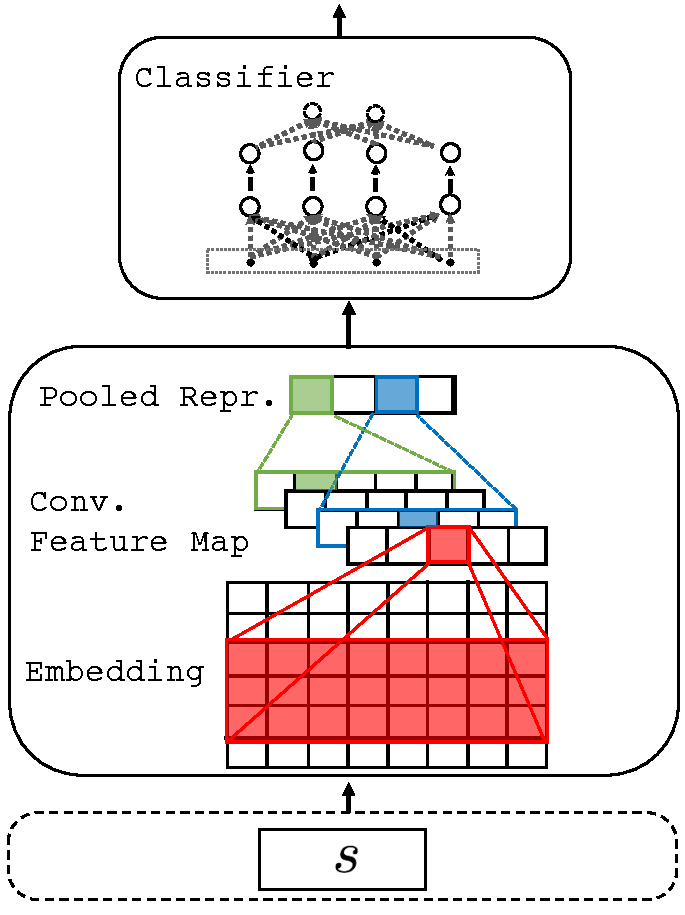
\includegraphics[width=0.35\textwidth]{03-part-02/chapter-05/figs_and_tables/fig_sentiment.pdf}
    \caption{The sentiment classifier used as \tch in \cws and \std in \fwl.}
    \label{fig:sentiment}
\end{figure}


\subsubsection{The \tnet in \cws and the \std in \fwl}
We use a convolutional model~\citep{Kim:2014} as the \tnet in \cws and the \std in \fwl, which is similar to the state-of-the-art model for Twitter sentiment classification from Semeval 2015 and 2016~\cite{Severyn:2015:SemEval,Deriu2016:SemEval,Deriu:2017,Severyn:2015:SIGIR}.

\mypar{The Representation Learning Layer} 
The representation learning layer in this task consists of an embedding function $\varepsilon: \mathcal{V} \rightarrow \mathbb{R}^{m}$, where $\mathcal{V}$ denotes the vocabulary set and $m$ is the number of embedding dimensions.

This function maps the sentence to a matrix $S \in \mathbb{R}^{m \times |s|}$, where each column represents the embedding of a word at the corresponding position in the sentence. We initialize the embedding matrix with word2vec embeddings~\cite{Mikolov:2013} pretrained on a collection of 50M tweets.

Matrix $S$ is passed through a convolution layer.  In this layer, a set of $f$ filters is applied to a sliding window of length $h$ over $S$ to generate a feature map matrix $O$. Each feature map $o_i$ for a given filter $F$ is generated by $o_i = \sum_{k,j}S[i:i+h]_{k,j} F_{k,j}$, where $S[i:i+h]$ denotes the concatenation of word vectors from position $i$ to $i+h$. The concatenation of all $o_i$ produces a feature vector $o \in \mathbb{R}^{|s|-h+1}$. The vectors $o$ are then aggregated over all $f$ filters into a feature map matrix $O \in \mathbb{R}^{f\times(|s|-h+1)}$.

We also add a bias vector $b \in R^f$ to the result of a convolution.
Each convolutional layer is followed by a non-linear activation function (we use ReLU\cite{Nair:2010}) which is applied element-wise. Afterward, the output is passed to the max pooling layer which operates on columns of the feature map matrix $O$ returning the largest value: $pool(o_i) : \mathbb{R}^{1\times(|s|-h+1)} \rightarrow \mathbb{R}$.

\mypar{The Supervision Layer.} 
This layer is a simple fully connected feed-forward network with $l$ hidden layers, followed by a softmax.  We employ the weighted cross entropy loss:
\begin{equation}
% \nonumber
\mathcal{L}_t = \sum_{i\in B_U} \tilde{c}_i \sum_{k \in K} - \tilde{y}_i^k \log (\hat{y}_i^k),
\end{equation}
where $B_U$ is a batch of instances from $U$, and $\tilde{c}_i$ is the confidence score of the weakly annotated instance $i$, and $K$ is a set of classes. 
The general schema of the \tnet (or \std) is illustrated in Figure~\ref{fig:sentiment}.

\subsubsection{The \wa}
\label{sentiment-WA}
The \wa for the sentiment classification task is a simple lexicon-based method~\citep{Hamdan:2013,Kiritchenko:2014}.
We use SentiWordNet03~\citep{Gaccianella:2010} to assign probabilities (positive, negative and neutral) for each token in set $\mathcal{D}_w$. We use a bag-of-words model for the sentence-level probabilities (i.e.\ just averaging the distributions of the terms), yielding a noisy label $\tilde{y}_i \in \mathbb{R}^{|K|}$, where $|K|=3$ is the number of classes.  We found empirically that using soft labels from the \wa works better than assigning a single hard label.


\subsubsection{The \cnet in \cws}
In this task, the \cnet is also a regresses and we use a simple fully connected feed-forward network. The target label $c_j$ for the \cnet is calculated by using the mean absolute difference of the strong label and the weak label: $c_j= 1-\frac{1}{|K|}\sum_{k\in K}|y_j^k - \tilde{y}_j^k|$, where $y_j$ is the one-hot encoding of the sentence label over all classes.


\subsubsection{The \tch in \fwl}
Similar to the ranking task, we use Gaussian Process as the \tch in order to generate soft labels. We pass the mean of $\mathcal{GP}$ through the same function $g(.)$ that is applied on the output of the \std network, where the $g(.)$ is softmax for the sentiment classification task.
Here in this task, $h(.)$ is an aggregation function that takes variance over several dimensions and outputs a single measure of variance. As a reasonable choice, the aggregating function $h(.)$ in the sentiment classification task (three classes) is \emph{mean} of variances over dimensions. 
In the \tch, linear combinations of different kernels are used. For the sentiment classification task, We use sparse variational GP for multiclass classification\footnote{\url{http://gpflow.readthedocs.io/en/latest/notebooks/multiclass.html}}~\citep{hensman2014scalable} with the following kernel:
\begin{equation}
k(x_i,x_j)=k_{\rm RBF}(x_i,x_j)+{k_{\rm Linear}}(x_i,x_j)+k_{\rm White}(x_i,x_j)
\end{equation}
where,
\begin{flalign*}
    \hspace{6em}
    &&k_{\rm RBF}(x_i,x_j) &= \exp{\left(\frac{\Vert x_i-x_j\Vert^2}{2l^2}\right)} & 
    \\
    &&k_{\rm Linear}(x_i,x_j) &= \sigma_0^2+x_i.x_j & \\
    &&k_{\rm White}(x_i,x_j) &= constant\_value, \quad \forall x_1=x_2 \text{ and } 0 \text{ otherwise} & 
\end{flalign*}

Similar to the ranking task, we set $l=1$ the length scale of RBF kernel, set $\sigma_0 = 0$  for the linear kernel, and set the number of clusters to $30$ in clustered $\mathcal{GP}$ algorithm.


\subsubsection{Collections}
We test our model on the twitter message-level sentiment classification of SemEval-15 Task 10B \citep{rosenthal:2015}. Datasets of SemEval-15 subsume the test sets from previous editions of SemEval, i.e. SemEval-13 and SemEval-14. Each tweet was preprocessed so that URLs and usernames are masked.

\mypar{Data with strong labels.} 
We use train (9,728 tweets) and development (1,654 tweets) data from SemEval-13 for training and SemEval-13-test (3,813 tweets) for validation.
To make your results comparable to the official runs on SemEval we us SemEval-14 (1,853 tweets) and  SemEval-15 (2,390 tweets) as test sets~\citep{rosenthal:2015, Nakov:2016}.

\mypar{Data with weak labels.}
We use a large corpus containing 50M tweets collected during two months for both, training the word embeddings and creating the weakly annotated set $\mathcal{D}_w$ using the lexicon-based method explained in Section~\ref{sentiment-WA}. 

\subsubsection{Experimental Setup.}
Similar to the document ranking task, we tuned hyper-parameters for the \tnet in \cws (and \std in the first step of \fwl) with respect to the strong labels of the validation set using batched GP bandits with an expected improvement acquisition function~\citep{Desautels:2014} and kept the optimal parameters fixed for all the other experiments.  
The size and number of hidden layers for the classifier and is selected from $\{32, 64, 128\}$.
We tested the model with both, $1$ and $2$ convolutional layers. The number of convolutional feature maps and the filter width is selected from $\{200,300\}$ and $\{ 3, 4, 5\}$, respectively. The initial learning rate and the dropout parameter were selected from $\{1E-3, 1E-5\}$ and $\{0.0, 0.2, 0.5\}$, respectively. We considered embedding sizes of $\{100, 200\}$ and the batch size in these experiments was set to $64$. ReLU~\citep{Nair:2010} is used as a non-linear activation function in \tnet (and \std).  Adam optimizer~\citep{Kingma:2014} is used for training, and \emph{dropout}~\citep{Srivastava:2014} as a regularizer.

In the rest of the chapter, we will present the main results of the introduced baseline methods and the proposed models, \cws and \fwl, 


\subsubsection{Results and Discussions} 
\begin{table}[!t]
            \renewcommand{\arraystretch}{1.1}
            \centering
            \caption{\label{tbl_main_sent}Performance ofof \cws and \fwl as well as the main baseline methods,described in Table~\ref{tbl_baselines}, for the sentiment classification task. 
            \pssmall{i} indicates that the improvements with respect to the baseline $i$ are statistically significant at the 0.05 level using the paired two-tailed t-test with Bonferroni correction.}
            \begin{tabular}{r l l l}
            \toprule
            & \textbf{Method} & \textbf{SemEval-14} & \textbf{SemEval-15}
            \\ \midrule
            \bf 1 & \bf \small{WA$_\text{Lexicon}$} 
            & 0.5141 & 0.4471
            \\ \midrule
           \bf  2 & \bf \small{$\text{NN}_{\text{S}}$} 
            & 0.6307\pssmall{1} & 0.5811\pssmall{13}
            \\
            \bf 3 & \bf \small{$\text{NN}_{\text{W}}$} 
            & 0.6719\pssmall{12} & 0.5606\pssmall{1} 
            \\ \midrule
            \bf 4 & \bf \small{$\text{NN}_{\text{W}\text{/S}^+}$} 
            & 0.7032\pssmall{12367} & 0.6319\pssmall{12367}
            \\
            \bf 5 & \bf \small{$\text{NN}_{\text{W}} \to \text{NN}_{\text{S}}$}
            & 0.7080\pssmall{12367} & 0.6441\pssmall{12367}
            \\
           \bf  6 & \bf \small{$\text{NN}_{\text{W}} \to \text{NN}^{\text{Sup}}_{\text{S}}$} 
            & 0.6875\pssmall{123} & 0.6193\pssmall{123}
            \\
            \bf 7 & \bf \small{$\text{NN}_{\text{W}} \to \text{NN}^{\text{Rep}}_{\text{S}}$}
            & 0.6932 \pssmall{123} & 0.6102\pssmall{123}
            \\ \midrule
            \bf 8 & \bf \small{\cws} 
            & 0.7362 \pssmall{1234567} & 0.6626\pssmall{1234567}
            \\
            \bf 13 & \bf \small{\fwl} 
            & \textbf{0.7470} \pssmall{12345678} & \textbf{0.6830}\pssmall{12345678}
            \\ \midrule
            \bf $\ast$ & \bf \small{SemEval$^\text{Best}$} 
            & 0.7162~\citep{Rouvier:2016} & 0.6618~\citep{Deriu2016:SemEval}
            \\\bottomrule
            \end{tabular}
\end{table}
We report Macro-F1, the official SemEval metric, in Table~\ref{tbl_main_sent}. 

Among all the baselines, \fwl is the best performing approach. \cws is also outperforms all the baselines. 

For this task, since the amount of data with strong labels are larger compared to the ranking task, the performance of $\text{NN}_{\text{S}}$ is acceptable. Alternately sampling from weak and strong data, i.e.  $\text{NN}_{\text{W}\text{/S}^+}$ gives better results than either of learning from just weak or just strong labels. However, pretraining on weak labels then fine-tuning both the supervision layer and the representation learning layer on strong labels, further improves the performance.  

Besides the baselines, we also report the best performing systems which are also convolution-based models (\citealt{Rouvier:2016} on SemEval-14; \citealt{Deriu2016:SemEval} on SemEval-15). Both \cws and \fwl outperform these methods.


\begin{table}[!t]
            \renewcommand{\arraystretch}{1.1}
            \centering
            \caption{\label{tbl_variants_sent_cws}Performance of the variants of the \cws on different datasets for the sentiment classification task. Baselines are described in Table~\ref{tbl_baselines}.}
            \begin{tabular}{r l l l}
            \toprule
            & Method & SemEval-14 & SemEval-15
            \\ \midrule
            8 & \small{\cws} 
            & 0.7362 & 0.6626
            \\
            9 & \small{\cws$_\text{JT+}$} 
            & 0.7310 & 0.6551
            \\
            10 & \small{\cws$_\text{ST}$} 
            & 0.7183 & 0.6501
            \\
            11 & \small{\cws$_\text{CT}$} 
            & \textbf{0.7363} & \textbf{0.6667}
            \\
            12 & \small{\cws$_\text{PT}$}
            & 0.7009 & 0.6118
            \\\bottomrule
            \end{tabular}
\end{table}
Similar to the ranking task, we have done an ablation study on \cws by trying different strategies for training \cws. The results of these experiments are presented in Table~\ref{tbl_variants_sent_cws}. \cws$_\text{CT}$ archives the highest performance among all the training strategies, however, as we discussed in Section~\ref{sec:res_and_disc_ranking}, it is not as efficient as \cws. 

In sentiment classification, compared to the ranking task, it is easier to estimate the confidence score of instances concerning the amount of available supervised data. Therefore, \cws$_\text{ST}$ improves the performance over $\text{NN}_{\text{S}}$ in Table~\ref{tbl_main_sent}. 


\begin{table}[!t]
            \renewcommand{\arraystretch}{1.1}
            \centering
            \caption{\label{tbl_variants_sent_fwl}Performance of \fwl against some of the baselines on different datasets for document ranking task. Baselines are described in Table~\ref{tbl_baselines}.}
            \begin{tabular}{r l c c}
            \toprule
            & \textbf{Method} & \textbf{SemEval-14} & \textbf{SemEval-15}
            \\ \midrule
            \bf 13 & \bf \small{\fwl} 
            & \textbf{0.7470} & \textbf{0.6830}
            \\
            \bf 14 & \bf \small{$\text{NN}_{\text{W}^\omega \to \text{NN}_\text{S}}$} 
            & 0.7166 & 0.6603
            \\
            \bf 15 & \bf \small{\fwlnospace$_{unsuprep}$} 
            & 0.6588  & 0.6954
            \\ 
            \bf 16 & \bf \small{\fwlnospace$\backslash\Sigma$} 
            & 0.7202 & 0.6590
            \\\bottomrule
            \end{tabular}
\end{table}
The results of a set of experiments we have done as ablation studies on \fwl is presented Table~\ref{tbl_variants_sent_fwl}. 

Having static weighting on the gradient updates, i.e. NN$_{\text{W}^\omega \to \text{S}}$, leads to the performance that is better than simple fine-tuning, i.e. $\text{NN}_{\text{W}} \to \text{NN}_{\text{S}}$ in Table~\ref{tbl_main_sent} .
%
For this task, similar to the ranking task, learning the representation in an unsupervised task independent fashion, i.e. \fwlnospace$_{unsuprep}$, does not lead to good results compared to the \fwl.
%
Similar to the ranking task, fine-tuning $\text{NN}_{\text{W}}$ based on labels generated by $\mathcal{GP}$ instead of data with strong labels, regardless of the confidence score, i.e. \fwl$\backslash\Sigma$, works better than standard fine-tuning. 
